\documentclass[../../../analisi-dei-requisiti.tex]{subfiles}

\begin{document}

\subsubsection{UUC4: Visualizza lista organizzazioni}%
\label{subs:UUC4}


\begin{figure}[H]
  \centering
  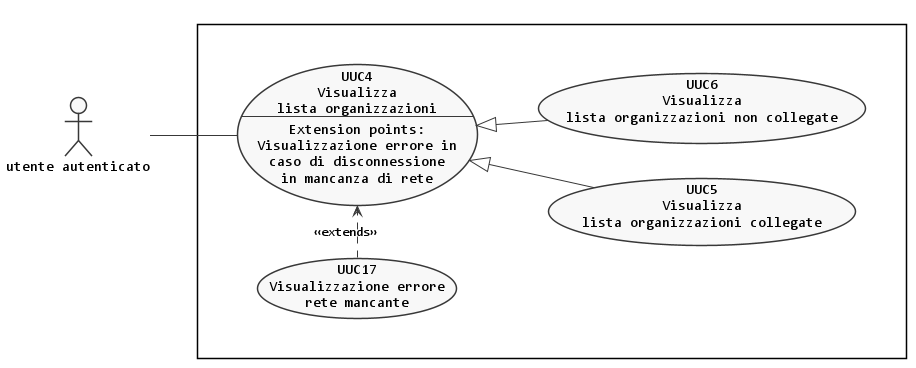
\includegraphics[width=150mm]{gestione-lista-organizzazioni.png}
  \caption{UUC4: Visualizza lista organizzazioni}%
  \label{fig:UUC4}
\end{figure}

\begin{description}
  \item[Caso d'uso:] UUC4;
  \item[Titolo:] Visualizza lista organizzazioni;
  \item[Attori primari:] utente autenticato;
  \item[Precondizione:] il sistema deve rendere disponibile la pagina relativa al recupero della lista delle organizzazioni;
  \item[Postcondizione:] l'utente visualizza la pagina relativa alla lista delle organizzazioni;
  \item[Scenario principale:]
        \begin{enumerate}
          \item l'utente ha la possibilità di recuperare una lista di organizzazioni alle quali si può collegare, o a cui è già collegato;
        \end{enumerate}
  \item[Estensioni:]
        \begin{enumerate}
          \item in caso di rete mancante, non possono essere eseguite queste operazioni e quindi verrà notificato un errore~\ref{subs:UUC17};
        \end{enumerate}
\end{description}



\subsubsection{UUC5: Visualizza lista organizzazioni collegate}%
\label{subs:UUC5}

\begin{figure}[H]
  \centering
  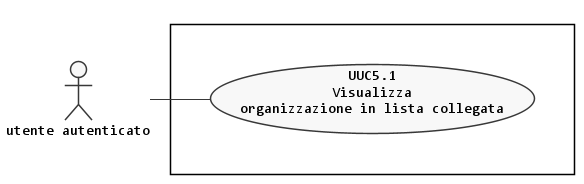
\includegraphics[width=100mm]{ visualizza-organizzazione-collegata.png}
  \caption{UUC5: Visualizza lista organizzazioni}%
  \label{fig:UUC5}
\end{figure}

\begin{description}
  \item[Caso d'uso:] UUC5;
  \item[Titolo:] Visualizza lista organizzazioni collegate;
  \item[Attori primari:] utente autenticato;
  \item[Precondizione:] il sistema deve rendere disponibile la pagina relativa al recupero della lista delle organizzazioni a cui l'utente è collegato;
  \item[Postcondizione:] l'utente visualizza la pagina relativa alla lista delle organizzazioni a cui è collegato;
  \item[Scenario principale:]
        \begin{enumerate}
          \item l'utente ha la possibilità di recuperare una lista di organizzazioni alle quali è collegato;
        \end{enumerate}
  \item[Estensioni:]
        \begin{enumerate}
          \item in caso di rete mancante, non possono essere eseguite queste operazioni e quindi verrà notificato un errore~\ref{subs:UUC17};
        \end{enumerate}
\end{description}

\subsubsection{UUC5.1: Visualizza informazioni organizzazione collegata}%
\label{subs:UUC5.1}

\begin{figure}[H]
  \centering
  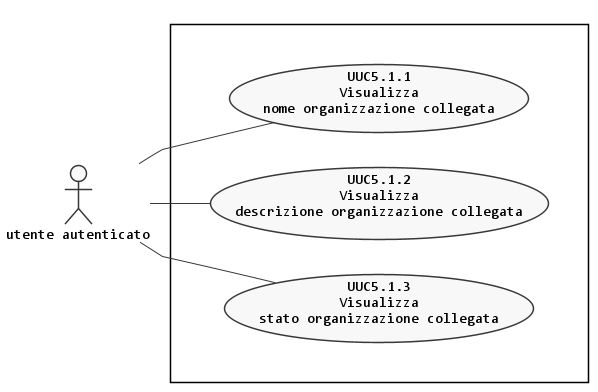
\includegraphics[width=100mm]{visualizza-info-organizzazione-collegata.png}
  \caption{UUC5.1: Visualizza informazioni organizzazione collegata}%
  \label{fig:UUC5.1}
\end{figure}

\begin{description}
  \item[Caso d'uso:] UUC5.1;
  \item[Titolo:] Visualizza informazioni organizzazione collegata;
  \item[Attori primari:] utente autenticato;
  \item[Precondizione:] il sistema deve rendere disponibile la pagina relativa al recupero della lista delle organizzazioni a cui l'utente è collegato;
  \item[Postcondizione:] l'utente visualizza le informazioni riguardo un'organizzazione a cui è collegato;
  \item[Scenario principale:]
        \begin{enumerate}
          \item l'utente ha la possibilità di visualizzare le informazioni riguardo un'organizzazione a cui è collegato;
        \end{enumerate}
  \item[Estensioni:]
        \begin{enumerate}
          \item in caso di rete mancante, non possono essere eseguite queste operazioni e quindi verrà notificato un errore~\ref{subs:UUC17};
        \end{enumerate}
\end{description}


\subsubsection{UUC5.1.1: Visualizza nome organizzazione collegata}%
\label{subs:UUC5.1.1}
\begin{description}
  \item[Caso d'uso:] UUC5.1.1;
  \item[Titolo:] Visualizza nome organizzazione collegata;
  \item[Attori primari:] utente autenticato;
  \item[Precondizione:] il sistema deve rendere disponibile la pagina relativa al recupero della lista delle organizzazioni a cui l'utente è collegato;
  \item[Postcondizione:] l'utente visualizza il nome di un'organizzazione a cui è collegato;
  \item[Scenario principale:]
        \begin{enumerate}
          \item l'utente ha la possibilità di visualizzare il nome di un'organizzazione a cui è collegato;
        \end{enumerate}
\end{description}

\subsubsection{UUC5.1.2: Visualizza descrizione organizzazione collegata}%
\label{subs:UUC5.1.2}
\begin{description}
  \item[Caso d'uso:] UUC5.1.2;
  \item[Titolo:] Visualizza descrizione organizzazione collegata;
  \item[Attori primari:] utente autenticato;
  \item[Precondizione:] il sistema deve rendere disponibile la pagina relativa al recupero della lista delle organizzazioni a cui l'utente è collegato;
  \item[Postcondizione:] l'utente visualizza la descrizione di un'organizzazione a cui è collegato;
  \item[Scenario principale:]
        \begin{enumerate}
          \item l'utente ha la possibilità di visualizzare la descrizione di un'organizzazione a cui è collegato;
        \end{enumerate}
\end{description}

\subsubsection{UUC5.1.3: Visualizza stato organizzazione collegata}%
\label{subs:UUC5.1.3}
\begin{description}
  \item[Caso d'uso:] UUC5.1.3;
  \item[Titolo:] Visualizza stato organizzazione collegata;
  \item[Attori primari:] utente autenticato;
  \item[Precondizione:] il sistema deve rendere disponibile la pagina relativa al recupero della lista delle organizzazioni a cui l'utente è collegato;
  \item[Postcondizione:] l'utente visualizza lo stato di un'organizzazione a cui è collegato;
  \item[Scenario principale:]
        \begin{enumerate}
          \item l'utente ha la possibilità di visualizzare lo stato (pubblico o privato) di un'organizzazione a cui è collegato;
        \end{enumerate}
\end{description}


\subsubsection{UUC6: Visualizza lista organizzazioni non collegate}%
\label{subs:UUC6}

\begin{figure}[H]
  \centering
  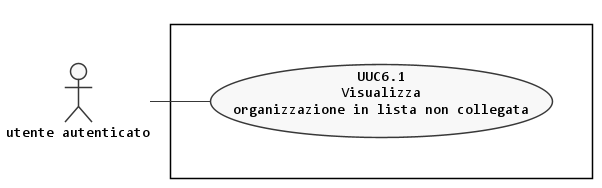
\includegraphics[width=100mm]{visualizza-organizzazione-non-collegata.png}
  \caption{UUC6: Visualizza lista organizzazioni non collegate}%
  \label{fig:UUC6}
\end{figure}

\begin{description}
  \item[Caso d'uso:] UUC6;
  \item[Titolo:] Visualizza lista organizzazioni non collegate;
  \item[Attori primari:] utente autenticato;
  \item[Precondizione:] il sistema deve rendere disponibile la pagina relativa al recupero della lista delle organizzazioni a cui l'utente non è collegato;
  \item[Postcondizione:] l'utente visualizza la pagina relativa alla lista delle organizzazioni a cui non è collegato;
  \item[Scenario principale:]
        \begin{enumerate}
          \item l'utente ha la possibilità di recuperare una lista di organizzazioni a cui non è collegato;
        \end{enumerate}
  \item[Estensioni:]
        \begin{enumerate}
          \item in caso di rete mancante, non possono essere eseguite queste operazioni e quindi verrà notificato un errore~\ref{subs:UUC17};
        \end{enumerate}
\end{description}

\subsubsection{UUC6.1: Visualizza informazioni organizzazione non collegata}%
\label{subs:UUC6.1}

\begin{figure}[H]
  \centering
  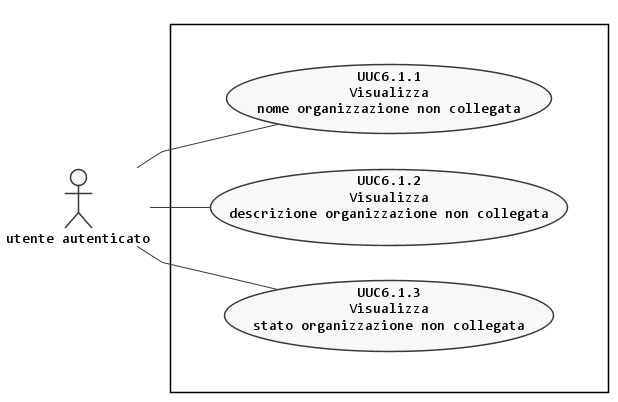
\includegraphics[width=100mm]{visualizza-info-organizzazione-non-collegata.png}
  \caption{UUC6.1: Visualizza informazioni organizzazione non collegata}%
  \label{fig:UUC6.1}
\end{figure}

\begin{description}
  \item[Caso d'uso:] UUC6.1;
  \item[Titolo:] Visualizza informazioni organizzazione non collegata;
  \item[Attori primari:] utente autenticato;
  \item[Precondizione:] il sistema deve rendere disponibile la pagina relativa al recupero della lista delle organizzazioni non collegate;
  \item[Postcondizione:] l'utente visualizza le informazioni riguardo un'organizzazione a cui non è collegato;
  \item[Scenario principale:]
        \begin{enumerate}
          \item l'utente ha la possibilità di visualizzare le informazioni riguardo un'organizzazione a cui non è collegato;
        \end{enumerate}
  \item[Estensioni:]
        \begin{enumerate}
          \item in caso di rete mancante, non possono essere eseguite queste operazioni e quindi verrà notificato un errore~\ref{subs:UUC17};
        \end{enumerate}
\end{description}


\subsubsection{UUC6.1.1: Visualizza nome organizzazione non collegata}%
\label{subs:UUC6.1.1}
\begin{description}
  \item[Caso d'uso:] UUC6.1.1;
  \item[Titolo:] Visualizza nome organizzazione non collegata;
  \item[Attori primari:] utente autenticato;
  \item[Precondizione:] il sistema deve rendere disponibile la pagina relativa al recupero della lista delle organizzazioni non collegate;
  \item[Postcondizione:] l'utente visualizza il nome di un'organizzazione a cui non è collegato;
  \item[Scenario principale:]
        \begin{enumerate}
          \item l'utente ha la possibilità di visualizzare il nome di un'organizzazione a cui non è collegato;
        \end{enumerate}
\end{description}

\subsubsection{UUC6.1.2: Visualizza descrizione organizzazione non collegata}%
\label{subs:UUC6.1.2}
\begin{description}
  \item[Caso d'uso:] UUC6.1.2;
  \item[Titolo:] Visualizza descrizione organizzazione non collegata;
  \item[Attori primari:] utente autenticato;
  \item[Precondizione:] il sistema deve rendere disponibile la pagina relativa al recupero della lista delle organizzazioni non collegate;
  \item[Postcondizione:] l'utente visualizza la descrizione di un'organizzazione a cui non è collegato;
  \item[Scenario principale:]
        \begin{enumerate}
          \item l'utente ha la possibilità di visualizzare la descrizione di un'organizzazione a cui non è collegato;
        \end{enumerate}
\end{description}

\subsubsection{UUC6.1.3: Visualizza stato organizzazione non collegata}%
\label{subs:UUC6.1.3}
\begin{description}
  \item[Caso d'uso:] UUC6.1.3;
  \item[Titolo:] Visualizza stato organizzazione non collegata;
  \item[Attori primari:] utente autenticato;
  \item[Precondizione:] il sistema deve rendere disponibile la pagina relativa al recupero della lista delle organizzazioni non collegate;
  \item[Postcondizione:] l'utente visualizza lo stato di un'organizzazione a cui non è collegato;
  \item[Scenario principale:]
        \begin{enumerate}
          \item l'utente ha la possibilità di visualizzare lo stato (pubblico o privato) di un'organizzazione a cui non è collegato;
        \end{enumerate}
\end{description}


\subsubsection{UUC7: Aggiornamento lista organizzazioni}%
\label{subs:UUC7}
\begin{description}
  \item[Caso d'uso:] UUC7;
  \item[Titolo:] Aggiornamento lista organizzazioni;
  \item[Attori primari:] utente autenticato;
  \item[Precondizione:] l'utente visualizza la lista delle organizzazioni;
  \item[Postcondizione:] l'utente ha aggiornato la lista delle organizzazioni;
  \item[Scenario principale:]
        \begin{enumerate}
          \item l'utente ha la possibilità di aggiornare la lista delle organizzazioni, e viene avvisato mediante \glossario{notifica} dell'applicazione mobile.
        \end{enumerate}
  \item[Estensioni:]
        \begin{enumerate}
          \item in caso di rete mancante, non può essere eseguito l'aggiornamento della lista di organizzazioni e quindi verrà notificato un errore~\ref{subs:UUC17}.
        \end{enumerate}
\end{description}






\end{document}
